\section{The universal enveloping algebra}
The following hold for this section alone: We fix an arbitrary field $k$ and a Lie algebra $\g$ over $k$. By a $k$-algebras we always mean an associative and unitary one, and homomorphisms of $k$-algebras have to respect the unit. The resulting category of $k$-algebras with homomorphisms of $k$-algebras between them will be denoted by $\cAlg{k}$.





\subsection{Definition, properties and construction}


\begin{defi}
 An \emph{universal enveloping algebra} of $\g$ is an $k$-algebra $\Ue(\g)$ together with a homomorphism of Lie algebras $\iota \colon \g \to \Ue(\g)$ such that for every $k$-Algebra $A$ and homomorphism of Lie algebras $\phi \colon \g \to A$ there exists a unique homomorphism of $k$-algebras $\Phi \colon \Ue(\g) \to A$ with $\phi = \Phi \circ \iota$, i.e.\ making the following diagram commute:
 \begin{center}
  \tikzsetnextfilename{universal_property_of_universal_enveloping_algebra}
  \begin{tikzpicture}[node distance = 5em]
   \node (g) {$\g$};
   \node[below of = g] (Ug) {$\Ue(\g)$};
   \node[right = 5em of Ug] (A) {$A$};
   \draw[->] (g) to node[left] {$\iota$} (Ug);
   \draw[->] (g) to node[above right] {$\phi$} (A);
   \draw[->, dashed] (Ug) to node[below] {$\Phi$} (A);
  \end{tikzpicture}
 \end{center}
\end{defi}


\begin{rem}
 As always with universal objects any two enveloping algebras of $\Ue(\g)_1$ with $\iota_1 \colon \g_1 \to \Ue(\g)_1$ and $\Ue(\g)_2$ with $\iota_2 \colon \g \to \Ue(\g)_2$ of $\g$ are isomorphic, and there exists a unique isomorphism $\varphi \colon \Ue(\g_1) \to \Ue(\g_2)$ with $\iota_2 = \varphi \colon \iota_1$, i.e.\ making the following diagram commute:
 \begin{center}
  \tikzsetnextfilename{uniqueness_of_universal_enveloping_algebra}
  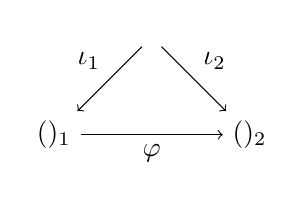
\begin{tikzpicture}[node distance = 5em]
   \node (g) {$\g$};
   \node[below left of = g] (U1) {$\Ue(\g)_1$};
   \node[below right of = g] (U2) {$\Ue(\g)_2$};
   \draw[->] (g) to node[above left] {$\iota_1$} (U1);
   \draw[->] (g) to node[above right] {$\iota_2$} (U2);
   \draw[->] (U1) to node[below] {$\varphi$} (U2);
  \end{tikzpicture}
 \end{center}
 Hence we will talk about \emph{the} universal enveloping algebra of $\g$.
\end{rem}


\begin{prop}\label{prop: representations of lie algebra isomorphic to modules over the universal enveloping algebra}
 Let $V$ be a vector space over $k$. Then there exists a bijection
 \begin{align*}
  \left\{
   \begin{tabular}{c}
    Representations of $\g$ \\
    $\rho \colon \g \to \gl(V)$
   \end{tabular}
  \right\}
  &\longrightarrow
  \left\{
   \begin{tabular}{c}
    $\Ue(\g)$-Modulstrukturen \\
    $\theta \colon \Ue(\g) \to \End_k(V)$
   \end{tabular}
  \right\}, \\
          \rho &\longmapsto   \hat{\rho}, \\
  \theta|_{\g} &\longmapsfrom \theta,
 \end{align*}
 where $\hat{\rho} \colon \Ue(\g) \to \End_k(V)$ is the $k$-algebra homomorphism induced by the homomorphism of Lie algebras $\rho \colon \g \to \gl(V)$ via the universial property of the universal enveloping algebra.
\end{prop}
\begin{proof}
 This is a direct consequence of the universal property of the universal enveloping algebra $\Ue(\g)$.
\end{proof}


\begin{rem}
 By Proposition \ref{prop: representations of lie algebra isomorphic to modules over the universal enveloping algebra} the category of representations of $\g$ is isomorphic to the category of modules over the universal enveloping algebra $\Ue(\g)$.
\end{rem}


\begin{rem}
 Given any two $k$-Lie algebras $\g_1$ and $\g_2$ then any homomorphism of Lie algebras $\phi \colon \g_1 \to \g_2$ induces a homomorphism of $k$-algebras $\phi^* \colon \Ue(\g_1) \to \Ue(\g_2)$ via the following commutative diagram:
 \tikzsetnextfilename{functoriality_of_the_universal_enveloping_algebra}
 \begin{center}
  \begin{tikzpicture}[node distance = 7em]
   \node (g1) {$\g_1$};
   \node[right of = g1] (g2) {$\g_2$};
   \node[below = 3em of g1] (Ug1) {$\Ue(\g_1)$};
   \node[below = 3em of g2] (Ug2) {$\Ue(\g_2)$};
   \draw[->] (g1) to node[above] {$\varphi$} (g2);
   \draw[->] (Ug1) to node[below] {$\varphi^*$} (Ug2);
   \draw[->] (g1) to node[left] {$\iota_1$} (Ug1);
   \draw[->] (g2) to node[right] {$\iota_2$} (Ug2);
  \end{tikzpicture}
 \end{center}
 Hence the assignment $\g \mapsto \Ue(g)$ of a Lie algebra to its universal eveloping algebra can be extended to a (covariant) functor $\Ue \colon \cLie{k} \to \cAlg{k}$. It is by the universal property of the universal enveloping algebra left adjoint to the functor $\cAlg{k} \to \cLie{k}$ which assignes each $k$-algebra its Lie algebra.
\end{rem}



\begin{lem}
 Let $T(\g) = \bigoplus_{n \in \N} \g^{\otimes n}$ be the tensor algebra and $\mc{I} \subseteq T(\g)$ the two-sided ideal generated by the element $x \otimes y - y \otimes x - [x,y]$ with $x,y \in \g$. The the quotient $\Ue(\g) \coloneqq T(\g)/\mc{I}$ together with the $k$-linear map
 \[
  \iota \colon \g \to \Ue(\g), \quad x \mapsto x + \mc{I}
 \]
 is an universal enveloping algebra of $\g$.
\end{lem}
\begin{proof}
 $\Ue(\g)$ is a $k$-algebra by construction and $\iota$ is a homomorphism of Lie algebras since for all $x,y \in \g$
 \begin{align*}
  [\iota(x),\iota(y)]
  &= [x + \mc{I}, y + \mc{I}]
  = (x + \mc{I})(y + \mc{I}) - (y + \mc{I})(x + \mc{I}) \\
  &= (x \otimes y - y \otimes x) + \mc{I}
  = [x,y] + \mc{I}
  = \iota([x,y]).
 \end{align*}
 Given any $k$-algebra $A$ and homomorphism of Lie algebras $\phi \colon \g \to A$ it can be uniquely extended to a homomorphism of $k$-algebras $\hat{\phi} \colon T(\g) \to A$ via
 \[
  \hat{\phi}(x_1 \otimes \dotsb \otimes x_n) = \phi(x_1) \dotsm \phi(x_n)
  \quad \text{for all $n \geq 0$ and $x_1, \dotsc, x_n \in \g$}.
 \]
 Because $\phi$ is not only $k$-linear but even a homomorphism of Lie algebras it follows that for all $x,y \in \g$
 \[
  \hat{\phi}(x \otimes y - y \otimes x)
  = \phi(x)\phi(y) - \phi(y)\phi(x)
  = [\phi(x),\phi(y)]
  = \phi([x,y])
  = \hat{\phi}([x,y])
 \]
 It follows that $\hat{\phi}(x) = 0$ for every $x \in \mc{I}$. Hence $\hat{\phi}$ factors through a unique homomorphism of $k$-algebras
 \[
  \Phi \colon \Ue(\g) \to A, \quad
  x_1 \otimes \dotsb \otimes x_n + \mc{I} \mapsto \phi(x_1) \dotsm \phi(x_n)
 \]
 for all $n \geq 0$ and $x_1, \dotsc, x_n \in \g$. For every $x \in \g$ it follows that
 \[
  (\Phi \circ \iota)(x)
  = \Phi(\iota(x))
  = \Phi(x + \mc{I}) 
  = \phi(x),
 \]
 which is why $\phi = \Phi \circ \iota$. That $\Phi$ is the unique homomorphism of $k$-algebras with this properties follows from the uniqueness of $\hat{\phi}$.
\end{proof}


\begin{cor}
 The homomorphism $\iota \colon \g \to \Ue(\g)$ is injective. As a $k$-algebra $\Ue(\g)$ is generated by $\iota(\g)$.
\end{cor}


\begin{rem}
 We will always identify $\g$ with its image under $\iota$.
\end{rem}





\subsection{Poincar\'{e}-Birkhoff-Witt}



\subsubsection{Graded $k$-algebras}


\begin{defi}\label{defi: graded algebras}
 A \emph{grading}, also called \emph{gradation}, of a $k$-algebra $A$ is a direct sum decomposition $A = \bigoplus_{i \in \N} A_i$ into linear subspaces such that
 \[
  A_i A_j \subseteq A_{i+j} \quad \text{for all $i,j \in \N$}.
 \]
 A \emph{graded $k$-algebra} is a $k$-algebra $A$ together with a grading $A = \bigoplus_{n \in \N} A_n$.
\end{defi}


\begin{rem}
 While a graded $k$-algebra is formally a pair $(A, (A_n)_{n \in \N})$ consisting of a $k$-algebra $A$ and a grading $A = \bigoplus_{n \in \N} A_n$ we will often just call $A$ a graded $k$-algebra without explicitily mentioning the grading. We also set $A_n \coloneqq 0$ for every $n < 0$.
\end{rem}


\begin{rem}
 Given any semigroup $(S,\cdot)$ an \emph{$S$-grading} of a $k$-algebra $A$ is a decomposition $A = \bigoplus_{s \in S} A_s$ into linear subspaces such that $A_s A_t \subseteq A_{s \cdot t}$ for all $s,t \in S$. An $S$-graded $k$-algebra is a $k$-algebra $A$ together with an $S$-grading $A = \bigoplus_{s \in S} A_s$. An graded $k$-algebra in the sense of Definition~\ref{defi: graded algebras} is then the special case of an $\N$-graded $k$-algebra.
\end{rem}


\begin{lem}
 Let $A$ be a graded $k$-algebra. Then $1 \in A_0$ and $A_0$ is a $k$-subalgebra.
\end{lem}
\begin{proof}
 Let $1 = \sum_{i \in \N} e_i$ with respect to $A = \bigoplus_{n \in \N} A_n$. Then for any $j \in \N$ and $a \in A_j$
 \[
  A_j \ni a
  = a \cdot 1
  = a \left( \sum_{i \in \N} e_i \right)
  = \sum_{i \in \N} \underbrace{a e_i}_{\in A_{i+j}},
 \]
 and it follows from the directness of the decomposition $A = \bigoplus_{n \in \N} A_n$ that $a = a e_0$. It follows that $a e_0 = a$ for every $a \in A$, hence $e_0$ is the unit of $A$.
 
 That $A_0$ is a linear subspace which is closed under the multiplication follows from the definition of a graded $k$-algebra. As it contains the unit of $A$ it is a $k$-subalgebra.
\end{proof}


\begin{expls}\label{expls: graded algebras}
 \begin{enumerate}[leftmargin=*]
  \item
   Any $k$-algebra $A$ becomes a graded $k$-algebra by setting $A_0 \coloneqq A$ and $A_i \coloneqq 0$ for every $i > 1$.
  \item
   The polynomial ring $A = k[x_1, \dotsc, x_n]$ is a graded $k$-algebra by setting
   \[
    A_d \coloneqq \vspan_k \{ x_1^{p_1} \dotsm x_n^{p_n} \mid p_1 + \dotsb + p_n = d\}
    \quad \text{for every $d \in \N$},
   \]
   i.e.\ $A_d$ consists of the homogeneous polynomials of degree $d$.
  \item
   Let $V$ be a $k$-vector space. Then the tensor algebra $T(V) = \bigoplus_{n \in \N} V^{\otimes n}$, the symmetric algebra $S(V) = \bigoplus_{n \in \N} S^n(V)$ and the exterior algebra $\Lambda(V) = \bigoplus_{n \in \N} \Lambda^n(V)$ carry the structure of a graded $k$-algebra via $T(V)_n \coloneqq V^{\otimes n}$, $S(V)_n \coloneqq S^n(V)$ and $\Lambda(V)_n \coloneqq \Lambda^n(V)$ for every $n \in \N$.
 \end{enumerate}
\end{expls}


\begin{defi}
 Let $A$ and $B$ be graded $k$-algebras. A homomorphism of $k$-algebras $\varphi \colon A \to B$ is called a \emph{homomorphism of graded $k$-algebras} if $\varphi(A_n) \subseteq B_n$ for every $n \in \N$, and the induced homomorphisms of vector spaces are denoted by $\varphi_n \colon A_n \to B_n$ for every $n \in \N$. An homomorphism of graded $k$-algebras is called an isomorphism if it is bijective.
\end{defi}


\begin{rem}
 If $A$ is a graded $k$-algebra then $\id_A$ is a homomorphism of graded $k$-algebras, and if $B$ and $C$ are two other graded $k$-algebras and $\varphi \colon A \to B$ and $\psi \colon B \to C$ homomorphisms of graded $k$-algebras then so is $\psi \colon \varphi \colon A \to C$. Hence the graded $k$-algebras together with the homomorphisms of graded $k$-algebras between them form a category, which will be refered to by $\cGrad{k}$.
\end{rem}


\begin{expl}
 \begin{enumerate}[leftmargin=*]
  \item
   For any vector space $V$ the two maps
   \begin{gather*}
    T(V) \to S(V), \quad x_1 \otimes \dotsb \otimes x_n \mapsto x_1 \dotsm x_n
   \shortintertext{and}
    T(V) \to \Lambda(V), \quad x_1 \otimes \dotsb \otimes x_n \mapsto x_1 \wedge \dotsb \wedge x_n
   \end{gather*}
   are homomorphisms of graded $k$-algebras.
  \item
   If $V$ is a finite dimensional vector space with basis $x_1, \dotsc, x_n$ the the isomorphism of $k$-algebras
   \[
    k[T_1, \dotsc, T_n] \to S(V), \quad T_i \mapsto x_i \quad \text{for every $i = 1, \dotsc, n$}
   \]
   is already an isomorphism of graded $k$-algebras.
 \end{enumerate}
\end{expl}


\begin{defi}
 Let $A$ be a graded $k$-algebra. A two-sided ideal $J \subseteq A$ is called \emph{homogeneous} if $J = \bigoplus_{n \in \N} (J \cap A_n)$. Equivalently, given any $x \in J$ with the decomposition $x = \sum_{n \in \N} x_n$ with respect to $A = \bigoplus_{n \in \N} A_n$ it follows that $x_n \in J$ for every $n \in \N$.
\end{defi}


\begin{lem}
 Let $A$ be a graded $k$-algebra and $J \subseteq A$ a two-sided homogeneous ideal. Then $A/J$ is a graded $k$-algebra via $(A/J)_n = A_n/(J \cap A_n)$ for every $n \in \N$ and the canonical projection $\pi \colon A \to A/J, a \mapsto a + J$ is a homomorphism of graded $k$-algebras.
\end{lem}
\begin{proof}
 This follows directly form the definition of a homogeneous ideal.
\end{proof}


\begin{lem}
 Let $A$ be a graded $k$-algebra, $J \subseteq A$ a two-sided ideal and call an element $x \in J$ \emph{homogeneous (in $J$)} if $x_n \in J$ for every $n \in \N$ where $x = \sum_{n \in \N} x_n$ with respect to $A = \bigoplus_{n \in \N} A_n$. Then $J$ is homogeneous if and only if $J$ is generated by elements which are homogeneous in $J$.
\end{lem}
\begin{proof}
 Let $I \coloneqq \{x \in J \mid \text{$x$ is homogeneous in $J$}\}$ be the linear subspace of elements which are homogeneous in $J$. If $x \in I$ then $x_n \in J$ for every $n \in \N$ where $x = \sum_{n \in \N} x_n$ with respect to $A = \bigoplus_{n \in \N} A_n$. Given $a \in A$ with $a = \sum_{m \in \N} a_m$ with respect to $A = \bigoplus_{m \in \N} A_m$ it follows that $a_m x_n \in J$ for all $m,n \in \N$ because $J$ is left ideal, and therefore $ax = \sum_{m,n \in \N} a_m x_n \in J$. Hence $I$ is a left ideal. In the same way it follows that $I$ is also a right ideal and hence already a two-sided ideal in $A$.
 
 The ideal $J$ is homogeneous if and only if any of its elements is homogeneous in $J$, i.e.\ if $I = J$, from which the statement follows.
\end{proof}


\begin{expls}
 \begin{enumerate}[leftmargin=*]
  \item
   If $A$ and $B$ are graded $k$-algebras and $\varphi \colon A \to B$ a homomorphism of graded $k$-algebras then $\ker \varphi$ is a homogeneous ideal.
  \item
   Let $V$ be any vector space. The two-sided ideal $I$ of $T(V)$ generated by the elements $x \otimes y - y \otimes x$ with $x,y \in V$ is a homogeneous ideal of $T(V)$. The same goes for the two-sided ideal $J$ generated by the elements $x \otimes x$ with $x \in V$. The resulting (graded) quotient algebras are $S(V)$ and $\Lambda(V)$.
 \end{enumerate}
\end{expls}



\subsubsection{Filtered $k$-algebras}


\begin{defi}
 A \emph{filtration} of a $k$-algebra $A$ is an increasing sequence
 \[
  A_{(0)}
  \subseteq A_{(1)}
  \subseteq A_{(2)}
  \subseteq \dotsb
  \subseteq A
 \]
 such that $A = \bigcup_{i \in \N} A_{(i)}$ and $A_{(i)} A_{(j)} \subseteq A_{(i+j)}$ for all $i,j \in \N$, as well as $1 \in A_{(0)}$. A \emph{filtered $k$-algebra} is a $k$-algebra $A$ together with a filtration $A = \bigcup_{n \in \N} A_{(n)}$.
\end{defi}


\begin{rem}
 As for graded $k$-algebras we will refer to a filtered $k$-algebra $A$ without explicitely mentioning the filtration. We also set $A_{(n)} \coloneqq 0$ for every $n < 0$.
\end{rem}


\begin{defi}
 Let $A$ and $B$ be filtered $k$-algebras. A homomorphism of $k$-algebras $\varphi \colon A \to B$ is called a \emph{homomorphism of filtered $k$-algebras} if $\varphi(A_{(n)}) \subseteq B_{(n)}$ for every $n \in \N$.
\end{defi}


\begin{rem}
 If $A$, $B$ and $C$ are filtered $k$-algebras then $\id_A$ is a homomorphism of filtered $k$-algebras and if $\varphi \colon A \to B$ and $\psi \colon B \to C$ are homomorphisms of filtered $k$-algebras then $\psi \circ \varphi$ is also a homomorphism of filtered $k$-algebras. It follows that filtered $k$-algebras together with homomorphisms of filtered $k$-algebras between them form a category, which will be refered to by $\cFilt{k}$.
\end{rem}


\begin{expls}
 \begin{enumerate}[leftmargin=*]
  \item
   Any graded $k$-algebra $A$ also carries the structure of an filtered $k$-algebra by setting $A_{(n)} \coloneqq \bigoplus_{i \leq n} A_i$ for every $n \in \N$. If $\varphi \colon A \to B$ is a homomorphism of graded $k$-algebras then it is also a homomorphism of filtered $k$-algebras. Hence this construction results into a functor $\flt \colon \cGrad{k} \to \cFilt{k}$.
  \item 
   If $A$ is a filtered algebra and $I \subseteq A$ any two-sided ideal then $A/I$ is a filtered $k$-algebra via $(A/I)_{(n)} \coloneqq \pi(A_{(n)})$ for every $n \in \N$, where $\pi \colon A \to A/I, a \mapsto a + I$ denotes the canonical projection.
  \item
   If $\g$ is a $k$-Lie algebra then $\Ue(\g)$ carries the structure of a filtered $k$-algebra induced by the filtration of $T(\g)$, which in turn is induced by the gradation of $T(\g)$. Explicitely
   \[
   \Ue(\g)_{(n)}
   = \vspan_k \{x_1 \dotsm x_m \mid m \in \N, m \leq n, x_1, \dotsc, x_m \in \g\}
   \quad\text{for every $n \in \N$}.
   \]
 \end{enumerate}
\end{expls}


\begin{lem}
 Let $A$ be a graded $k$-algebra and set $B_n \coloneqq A_n/A_{n-1}$ for every $n \in \N$. Then for all $n,m \in \N$ the map
 \[
  B_n \times B_m \to B_{n+m}, ([a], [b]) \mapsto [ab]
 \]
 is well-defined and bilinear.
\end{lem}
\begin{proof}
 Let $a, a' \in A_n$ and $b, b' \in A_m$ with $[a] = [a']$ and $[b] = [b']$. Then $ab, a'b' \in A_{n+m}$ and because $[a] = [a']$ and $[b] = [b']$ it follows that $a-a' \in A_{n-1}$ and $b-b' \in A_{m-1}$. Therefore
 \[
  ab
  = (a'+(a-a'))(b'+(b-b'))
  = a'b' + \underbrace{(a-a')b'}_{\in A_{n+m-1}} + \underbrace{a'(b-b')}_{\in A_{n+m-1}} + \underbrace{(a-a')(b-b')}_{\in A_{n+m-2}}
 \]
 and thus $[ab] = [a'b']$.
\end{proof}


\begin{defi}
 Let $A$ be a filtered $k$-algebra. Its \emph{associated graded $k$-algebra} is the graded $k$-algebra consisting of the underlying vector space $\gr(A) \coloneqq \bigoplus_{n \in \N} \gr_n(A)$ with $\gr_i(A) \coloneqq A_{(i)} / A_{(i-1)}$ for every $i \in \N$ and the multiplication $\gr(A) \times \gr(A) \to \gr(A)$ induced by the well-defined bilinear maps
 \[
  \gr_n(A) \times \gr_m(A) \to \gr_{n+m}(A), \quad
  ([a],[b]) \to [ab]
  \quad\text{for all $n,m \in \N$}.
 \]
 together with the grading given by $\gr(A)_n \coloneqq \gr_n(A)$ for every $n \in \N$.
\end{defi}


\begin{rem}
 If $A$ and $B$ are filtered $k$-algebras and $\varphi \colon A \to B$ is a homomorphism of filtered $k$-algebras then $\varphi$ induces a $k$-linear map $\varphi_n \colon \gr(A)_n \to \gr(B)_n, [a] \mapsto [\varphi(a)]$ for every $n \in \N$, which result in a homomorphism of graded $k$-algebras
 \[
  \gr(\varphi) \coloneqq \bigoplus_{n \in \N} \varphi_n \colon \gr(A) \to \gr(B),
  \quad
  \sum_{n \in \N} a_n \mapsto \sum_{n \in \N} \varphi(a_n).
 \]
 Hence $\gr$ can be seen as a functor $\gr \colon \cFilt{k} \to \cGrad{k}$.
\end{rem}


\begin{expls}
 \begin{enumerate}[leftmargin=*]
  \item
   If $A$ is a graded $k$-algebra then $\gr(\flt(A))$ is naturally isomorphic to $A$ in the following way: The filtration on $\flt(A)$ is given by $A_{(n)} = \bigoplus_{i \leq n} A_i$ for every $n \in \N$. Hence there is for every $n \in \N$ an isomorphism of vector spaces
   \[
    \varphi_n \colon A_n \to A_{(n)}/A_{(n-1)} = \gr(\flt(A))_n, \quad a \mapsto [a].
   \]
   Combining these isomorphisms results in an isomorphism of graded $k$-algebras
   \[
    \bigoplus_{n \in \N} \varphi_n \colon
    \bigoplus_{n \in \N} A_n \to \bigoplus_{n \in \N} \gr(\flt(A))_n, \quad
    \sum_{n \in \N} a_n \mapsto \sum_{n \in \N} [a_n].
   \]
   We will therefore identify $A$ with $\gr A$ in the above way.
  \item
   Let $\g$ be a $k$-Lie algebra. The canonical projection
   \[
    \pi \colon T(\g) \to \Ue(\g), \quad x_1 \otimes \dotsb \otimes x_n \to x_1 \dotsm x_n
    \quad \text{for every $n \in \N$ and all $x_1, \dotsc, x_n \in \g$}
   \]
   is a homomorphism of filtered $k$-algebras, where the filtration of $T(\g)$ is induced by the gradation discussed in Examples \ref{expls: graded algebras}. Hence it induces a homomorphism of graded $k$-algebras
   \[
    \gr(\pi) \colon T(\g) \to \gr(\Ue(\g)),
   \]
   where $T(\g)$ is identified with $\gr(T(\g))$ as above. This homomorphism maps an element $x_1 \otimes \dotsb \otimes x_n$ with $x_1, \dots, x_n \in \g$ to the residue class $[x_1 \dotsm x_n] \in \gr(\Ue(\g))_n$.
 \end{enumerate}
\end{expls}



\subsubsection{The Poincar\'{e}-Birkhoff-Witt theorem}
For this subsection we fix some $k$-Lie algebra $\g$ with basis $(x_i)_{i \in I}$ where $(I, \leq)$ is a totally ordered index set. Before stating and proving the \emph{Poincar\'{e}-Birkhoff-Witt theorem} (PBW) we fix some notation which we will only use in this subsection.


\begin{defi}
 Let $\mc{I}_n \coloneqq \{(i_1, \dotsc, i_n) \mid i_1, \dotsc, i_n \in I, \; i_1 \leq \dotsb \leq i_n\}$ for every $n \in \N$ and set $\mc{I} \coloneqq \bigcup_{n \in \N} \mc{I}_n$. For every $\alpha = (i_1, \dotsc, i_n) \in I^n$ with $n \in \N$ let $x_\alpha \coloneqq x_{i_1} \dotsm x_{i_n} \in \Ue(\g)$.
\end{defi}


\begin{rem}
 Notice that $\mc{I}_0$ contains the empty tupel.
\end{rem}


\begin{thrm}[PBW (concrete version)] \label{thrm: pbw concrete}
 The familiy $(x_\alpha \mid \alpha \in \mc{I})$ is a $k$-basis of $\Ue(\g)$.
\end{thrm}


\begin{rem}
 The basis $(x_\alpha \mid \alpha \in \mc{I})$ can also be written as
 \[
  \left(
   x_{i_1}^{p_1} \dotsm x_{i_n}^{p_n}
  \mid
   n \in \N,\;
   i_1, \dotsc, i_n \in I,\;
   i_1 < \dotsb < i_n,\;
   p_1, \dotsc, p_n \geq 1
  \right).
 \]
\end{rem}


\begin{expl}
 If $\g$ is a finite dimensional $k$-Lie algebra with basis $x_1, \dotsc, x_n$ then $\Ue(\g)$ has a basis given by $(x_1^{p_1} \dotsm x_n^{p_n} \mid p_1, \dotsc, p_n \in \N)$. In particular a basis of $\Ue(\sll_2(k))$ is given by $(e^\ell h^m f^n \mid \ell, m ,n \in \N)$.
\end{expl}


\begin{lem}\label{lem: pbw concrete generating part}
 The collection $(x_\alpha \mid \alpha \in \mc{I})$ generates $\Ue(\g)$ as a vector space.
\end{lem}
\begin{proof}
 To show that $(x_\alpha \mid \alpha \in \mc{I})$ generates $\Ue(\g)$ as a vector space it sufficies to show that $\mc{B}_n \coloneqq (x_\alpha \mid m \leq n, \alpha \in \mc{I}_m)$ generates $\Ue(\g)_{(n)}$ as a vector space, which will be shown by induction over $n \in \N$: For $n = 0$ this is clear as $\Ue(\g) = k$ is one-dimensional and thus spanned by $x_{(\;)}$, the monomial corresponding to the empty tupel.
 
 Suppose that the statement holds for some $n \in \N$. Then $\Ue(\g)_{(n+1)}$ is generated as a vector space as a by the monomials $(x_{(i_1, \dotsc, i_n)} \mid m \leq n+1, \; i_1, \dotsc, i_m \in I)$. Therefore it sufficies to express these monomials in terms of $\mc{B}_{n+1}$. By induction hypothesis is it enough to check this for the monomials $(x_{(i_1, \dotsc, i_{n+1})} \mid i_1, \dotsc, i_{n+1} \in I)$. For this let $\alpha = (i_1, \dotsc, i_{n+1})$ be some fixed multiindex with $i_1, \dotsc, i_{n+1} \in I$.
 
 For any two $x,y \in \g$ one has $xy = yx + [x,y]$ with $[x,y] \in \Ue(\g)_{(1)}$. Hence there exists for any permutation $\sigma \in S_{n+1}$ a linear combination $R_\sigma \in \Ue(\g)_{(1)}$ with
 \[
  x_\alpha
  = x_{i_1} \dotsm x_{i_{n+1}}
  = x_{i_{\sigma(1)}} \dotsm x_{i_{\sigma(n+1)}} + R_\sigma
  = x_{(i_{\sigma(1)}, \dotsc, x_{\sigma(n+1)})} + R_\sigma.
 \]
 Let $\sigma \in S_{n+1}$ be a permutation with $i_{\sigma(1)} \leq \dotsb \leq i_{\sigma(n+1)}$. By induction hypothesis $R_\sigma \in \Ue(\g)_{(n)}$ can be expressed as a linear combination of the monomials $\mc{B}_n$. Hence $x_\alpha = x_{(i_{\sigma(1)}, \dotsc, i_{\sigma(n+1)})} + R_\sigma$ can be expressed as a linear combination of the monomials $\mc{B}_{n+1}$ because $x_{(i_{\sigma(1)}, \dotsc, i_{\sigma(n+1)})}$ is one of them.
\end{proof}


\begin{proof}[Proof of PBW (concrete version)]
 By Lemma~\ref{lem: pbw concrete generating part} the collection $(x_\alpha \mid \alpha \in \mc{I})$ generates $\Ue(\g)$ as a vector space, so all that’s left to show is that it is linearly independent.
 
 Let $V \coloneqq k[Z_i \mid i \in I]$ and for every $n \in \N$ let $V_{(n)}$ be the polynomials of degree $\leq n$. For every $n \in \N$ and $\alpha = (i_1, \dotsc, i_n) \in I^n$ write $Z_\alpha \coloneqq Z_{i_1} \dotsm Z_{i_n}$. If $i \in I$ and $\alpha = (i_1, \dotsc, i_n) \in I^n$ then write $i \leq \alpha$ if $i \leq i_j$ for every $j = 1, \dotsc, n$. Also set $i \cdot \alpha = (i, i_1, \dotsc, i_n) \in I^{n+1}$.
 
 To show that $(x_\alpha \mid \alpha \in \mc{I})$ is linearly independent $V$ will be given the structure of a representation of $\g$ such that
 \[
  x_i.Z_\alpha = Z_{i \cdot \alpha}
  \quad \text{for every $i \in I$ and $\alpha \in \mc{I}$ with $i \leq \alpha$}.
 \]
 Then for the corresponding $\Ue(\g)$-module structure on $V$ it follows that
 \[
  x_\alpha \cdot 1
  = x_\alpha \cdot Z_{(\;)}
  = Z_\alpha
  \quad \text{for every $\alpha \in \mc{I}$}
 \]
 where $1 \in V = k[Z_i \mid i \in I]$ and $(\;)$ denotes the empty tupel. Because $(Z_\alpha \mid \alpha \in \mc{I})$ is linearly independent it then follows that $(x_\alpha \mid \alpha \in \mc{I})$ is linearly independent. The existence of such an action follows from the following:
 
 \begin{claim*}
  There exists a unique sequence $(\varphi_n)_{n \in \N}$ of bilinear maps
  \[
   \varphi_n \colon \g \times V_{(n)} \to V_{(n+1)}, \quad (x,p) \mapsto x.p
  \]
  satisfying the following conditions:
  \begin{enumerate}
   \item\label{enum: pbw restriction coincides}
    The restriction of $\varphi_{n+1}$ to $\g \times V_{(n)}$ coincides with $\varphi_n$ for every $n \in \N$
   \item\label{enum: pbw essential condition}
    $x_i.Z_\alpha = Z_{i \cdot \alpha}$ for every $i \in I$ and $\alpha \in \mc{I}$ with $i \leq \alpha$.
   \item\label{enum: pbw representation of lie algebra}
    $x_i.x_j.Z_\alpha - x_j.x_i.Z_\alpha = [x_i, x_j].Z_\alpha$ for all $i,j \in I$ and every $\alpha \in \mc{I}$.
   \item\label{enum: pbw technical detail for construction}
    $x_i.Z_\alpha - Z_{i \cdot \alpha} \in V_{(n)}$ for every $n \in \N$, $i \in I$ and $\alpha \in \mc{I}_n$.
   \end{enumerate}
   (Condition \ref{enum: pbw restriction coincides} actually follows from the other conditions by the uniqueness of the sequence $(\varphi_n)_{n \in \N}$. See \cite[\S 17.4]{Humphreys} for more details.)
 \end{claim*}
 \begin{proof}
  Notice thet the notation $x.p$ with $x \in \g$ and $p \in V$ is unambiguous by condition \ref{enum: pbw restriction coincides}. The maps $\varphi_n$ will be defined by induction over $n$:
  
  As $V_{(0)}$ is one-dimensional and spanned by $1 = Z_{(\;)}$ it follows from condition \ref{enum: pbw essential condition} that $x_i.1 = x_i \cdot Z_{(\;)} = Z_{i \cdot (\;)} = Z_i$ for every $i \in I$. This defines $\varphi_0$ uniquely. Conditions \ref{enum: pbw essential condition} and \ref{enum: pbw technical detail for construction} hold by construction and the conditions \ref{enum: pbw restriction coincides} and \ref{enum: pbw representation of lie algebra} do not affect $\varphi_0$.
  
  Let $n \in \N$ and suppose $\varphi_m$ is constructed for every $m \leq n$. By condition \ref{enum: pbw restriction coincides} all that is left to define is $x_i.Z_\alpha$ for $\alpha \in \mc{I}_{n+1}$. If $i \leq \alpha$ then $x_i.Z_\alpha = Z_{i \cdot \alpha}$ by condition \ref{enum: pbw essential condition}.
  
  If $i > \alpha$ then there exists $\beta \in \mc{I}_n$ and $j \in I$ with $\alpha = j \cdot \beta$ such that $i > j$ and $j \leq \beta$. If condition \ref{enum: pbw representation of lie algebra} was to hold for $\varphi_{n+1}$ it follows that
  \begin{equation}\label{eqn: action defined as lie action}
   x_i.Z_\alpha
   = x_i.x_j.Z_\beta
   = x_j.x_i.Z_\beta + [x_i, x_j].Z_\beta.
  \end{equation}
  Because $\beta \in \mc{I}_n$ the term $[x_i, x_j].Z_\beta$ in the above sum is already defined. Because $x_i.Z_\beta \equiv Z_{i \cdot \beta} \pmod{V_{(n)}}$ there exists some $Y \in V_{(n)}$ with $x_i.Z_\beta = Z_{i \cdot \beta} + Y$. Let $\gamma \in \mc{I}_{n+1}$ be defined by taking $\beta$ and inserting $i$ at the right position. Then $Z_\gamma = Z_{i \cdot \beta}$. Because $j < i$ and $j \leq \beta$ it follows that $j \leq \gamma$ and therefore 
  \[
   x_j.Z_{i \cdot \beta}
   = x_j.Z_\gamma
   = Z_{i \cdot \gamma}
   = Z_{i \cdot (j \cdot \beta)}
   = Z_{i \cdot \alpha}
  \]
  Because every summand in
  \begin{equation}\label{eqn: I really wish Humphreys had explained this}
   \begin{aligned}
    x_i.Z_\alpha
    = x_j.x_i.Z_\beta + [x_i, x_j].Z_\beta
    &= x_j.(Z_{i \cdot \beta} + Y) + [x_i, x_j].Z_\beta \\
    &= Z_{i \cdot \alpha} + x_j.Y + [x_i, x_j].Z_\beta
   \end{aligned}
  \end{equation}
  is defined it follows that $\varphi_{n+1}$ is uniquely defined.
  
  Conditions \ref{enum: pbw restriction coincides} and \ref{enum: pbw essential condition} hold for $\varphi_{n+1}$ by construction. Condition \ref{enum: pbw technical detail for construction} holds for $i \leq \alpha$ by condition \ref{enum: pbw essential condition} and for $i > \alpha$ by \eqref{eqn: I really wish Humphreys had explained this} because $x_j.Y \in V_{(n+1)}$ and $[x_i, x_j].Z_\beta \in V_{(n+1)}$.
  
  It remains to check Condition \ref{enum: pbw representation of lie algebra} for $\varphi_{n+1}$, i.e.\ when $i,j \in I$ and $\alpha \in \mc{I}_n$. For $i = j$ this follows from the Lie bracket being alternating. Suppose that $i \neq j$. By the Lie bracket is antisymmetric it can be w.l.o.g.\ assumed that $i < j$.
  
  If $i \leq \alpha$ then $x_j.x_i.Z_\alpha$ is defined above by using \eqref{eqn: action defined as lie action} (where $\beta$ has to be replaced by $\alpha$ and $i$ and $j$ have to be switched), hence condition \ref{enum: pbw essential condition} holds in this case by construction. Notice that if $j \leq \alpha$ then also $i \leq \alpha$ because $i < j$.
  
  Hence the only case left is $i \nleq \alpha$. By the above it then follows that also $j \nleq \alpha$. As this cannot happen for $n = 0$ it can be w.l.o.g.\ assumed that $n \geq 1$. Let $k \in I$ and $\beta \in \mc{I}_{n-1}$ with $\alpha = k \cdot \beta$. Because condition \ref{enum: pbw representation of lie algebra} holds for $\varphi_n$ it follows that
  \begin{align*}
   x_i.x_j.Z_\alpha
   = x_i.x_j.x_k.Z_\beta
   &= x_i.(x_k.x_j.Z_\beta + [x_j, x_k].Z_\beta) \\
   &= x_i.x_k.x_j.Z_\beta + x_i.[x_j, x_k].Z_\beta
  \end{align*}
  Because $k < j$ and $k \leq \beta$ it follows from the previous discussed cases that
  \[
   x_i.x_k.(x_j.Z_\beta)
   = x_k.x_i.(x_j.Z_\beta) + [x_i, x_k].(x_j.Z_\beta).
  \]
  Combining the above results in the equality
  \[
   x_i.x_j.Z_\alpha
   = x_k.x_i.x_j.Z_\beta + [x_i, x_k].x_j.Z_\beta + x_i.[x_j, x_k].Z_\beta
  \]
  By switching $i$ and $j$ in the above calculations it also follows that 
  \[
   x_j.x_i.Z_\alpha
   = x_k.x_j.x_i.Z_\beta + [x_j, x_k].x_i.Z_\beta + x_j.[x_i, x_k].Z_\beta
  \]
  By using that condition \ref{enum: pbw representation of lie algebra} holds for $\varphi_n$ it follows from these two equalities and the Jacobi identity that
  \begin{align*}
        x_i.x_j.Z_\alpha - x_j.x_i.Z_\alpha 
   =&\, x_k.x_i.x_j.Z_\beta + [x_i, x_k].x_j.Z_\beta + x_i.[x_j, x_k].Z_\beta \\
    &\, - x_k.x_j.x_i.Z_\beta - [x_j, x_k].x_i.Z_\beta - x_j.[x_i, x_k].Z_\beta \\
   =&\, x_k.[x_i, x_j].Z_\beta + [[x_i, x_k], x_j].Z_\beta +  [x_i,[x_j,x_k]].Z_\beta \\
   =&\, x_k.[x_i, x_j].Z_\beta - [x_k, [x_i, x_j]].Z_\beta
   =    [x_i, x_j].x_k.Z_\beta
   =    [x_i, x_j].Z_\alpha.
  \qedhere
  \end{align*}
 \end{proof}
 This finishes the proof. 
\end{proof}


\begin{thrm}[PBW (abstract version)] \label{thrm: pbw abstract}
 Let $\g$ be a Lie algebra over $k$ and denote by $\pi$ the canonical projection
 \[
  \pi \colon T(\g) \to \Ue(\g), \quad
  x_1 \otimes \dotsb \otimes x_n \mapsto x_1 \dotsm x_n
  \quad \text{for all $x_1, \dotsc, x_n \in \g$}.
 \]
 Then the two homomorphisms of graded $k$-algebras $\gr(\pi) \colon T(\g) \to \gr(\Ue(\g))$ and
 \[
  \pi' \colon T(\g) \to S(\g), \quad 
  x_1 \otimes \dotsb \otimes x_n \mapsto x_1 \dotsm x_n
  \quad \text{for all $x_1, \dotsc, x_n \in \g$}
 \]
 have the same kernel and thus induce an isomorphism of graded algebras
 \begin{equation}\label{eqn: induced isomorphism of graded algebras}
  \varphi \colon S(\g) \to \gr(\Ue(\g)), \quad
  x_1 \dotsm x_n \mapsto [x_1 \dotsm x_n]
  \quad \text{for all $x_1, \dotsc, x_n \in \g$}.
 \end{equation}
\end{thrm}


\begin{rem}
 Notice that the two multiplications in \eqref{eqn: induced isomorphism of graded algebras} live in different $k$-algebras.
\end{rem}


\begin{prop}
 The concrete version and the abstract versions of the PBW-theorem are equivalent.
\end{prop}
\begin{proof}
 For $x, y \in \g$ it follows from the definition of $\gr(\pi)$ that
 \[
  \gr(\pi)(x \otimes y - y \otimes x) = [xy-yx] \in \gr(\Ue(\g))_2,
 \]
 with representative $xy-yx \in \Ue(\g)_{(2)}$. By the definition of $\Ue(\g)$ it follows that already \mbox{$xy-xy = [x,y] \in \Ue(\g)_{(1)}$}. Hence it follows for the residue class of $xy-yx$ in $\gr(\Ue(\g))_2 = \gr(\Ue(\g))_{(2)}/\gr(\Ue(\g))_{(1)}$ that $[xy-yx] = [[x,y]] = [0] = 0$. Hence $\gr(\pi)(x \otimes y - y \otimes x) = 0$.
 
 As the kernel of $\pi'$ is generated by the element $x \otimes y - y \otimes x$ with $x,y \in \g$ it follows that $\pi'$ factorizes through a homomorphism of graded $k$-algebras $\varphi$ as in Theorem~\ref{thrm: pbw abstract}.
 
 (concrete $\Rightarrow$ abstract) The algebra $\Ue(\g)$ has a basis $(x_\alpha \mid \alpha \in \mc{I})$ It follows that $\gr(\Ue(\g))_n$ has a basis given by the residue classes $([x_\alpha] \mid \alpha \in \mc{I}_n)$. The linear subspace $S(\g)_n$ has a basis $(x_1 \dotsm x_n \mid (i_1, \dotsc, i_n) \in \mc{I}_n)$ which is mapped by $\varphi_n$ to the above basis of $\gr(\Ue(\g))_n$. Hence $\varphi_n$ is an isomorphism for every $n \in \N$, which is why $\varphi$ is an isomorphism.
 
 (abstract $\Rightarrow$ concrete) As $(x_\alpha \mid \alpha \in \mc{I})$ generates $\Ue(\g)$ as a vector spaces by Lemma~\ref{lem: pbw concrete generating part} it sufficies to show that this collection is linearly independent. Suppose otherwise. Then there exists some minimal $n \in \N$ such that $(x_\alpha \mid m \leq n, \alpha \in \mc{I}_m)$ is linearly dependent. Hence there exists a non-trivial linear combination
 \[
  0 = \sum_{m=0}^n \sum_{\alpha \in \mc{I}_m} \lambda_\alpha x_\alpha
 \quad
 \text{where $\lambda_\alpha = 0$ for all but finitely many $\alpha \in \bigcup_{m=0}^n \mc{I}_m$}.
 \]
 From this it follows that
 \[
  0
  = \sum_{m=0}^n \sum_{\alpha \in \mc{I}_m} \lambda_\alpha x_\alpha
  \equiv \sum_{\alpha \in \mc{I}_n} \lambda_\alpha x_\alpha
  \mod \Ue(g)_{(n-1)}
 \]
 and hence that the equality $\sum_{\alpha \in \mc{I}_n} \lambda_\alpha [x_\alpha] = 0$ holds in $\gr(\Ue(\g))_n = \Ue(\g)_{(n)}/\Ue(\g)_{(n-1)}$. By the minimality of $n$ it follows that this is a non-trivial linear combination in $\gr(\Ue(\g))_n$, so $([x_\alpha] \mid \alpha \in \mc{I}_n)$ in $\gr(\Ue(\g))_n$ is linearly dependent.
 
 By assumption $\varphi$ is a homomorphism of graded $k$-algebras and therefore $\varphi_n$ is an isomorphism of vector spaces. As the basis $(x_{i_1} \dotsm x_{i_n} \mid (i_1, \dotsc, i_n) \in \mc{I}_n)$ of $S(\g)_n$ is mapped by $\varphi_n$ bijectively to $([x_\alpha] \mid \alpha \in \mc{I}_n)$ it follows that this is a basis of $\gr(\Ue(\g))_n$, contradicting the linearly dependency.
\end{proof}





\subsection{Free Lie algebras}


\begin{defi}
 Let $X$ be a set. A \emph{free $k$-Lie algebra on $X$} is a Lie algebra $F(X)$ together with a map $\iota \colon X \to F(X)$ such that for every Lie algebra $\g$ and map $\phi \colon X \to \g$ there exists a unique homomorphism of Lie algebras $\Phi \colon F(X) \to \g$ with $\phi = \Phi \circ \iota$, i.e.\ making the following diagram commute:
 \tikzsetnextfilename{universal_property_of_the_free_Lie_algebra}
 \begin{center}
  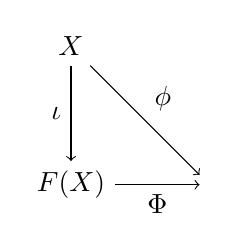
\begin{tikzpicture}[node distance = 5em]
   \node (X) {$X$};
   \node (FX)[below of = X] {$F(X)$};
   \node (g)[right of = FX] {$\g$};
   \draw[->] (X) to node[left] {$\iota$} (FX);
   \draw[->] (X) to node[above right] {$\phi$} (g);
   \draw[->] (FX) to node[below] {$\Phi$} (g);
  \end{tikzpicture}
 \end{center}
\end{defi}


\begin{rem}
 As usual with free objects it follows that any two free Lie algebras over a set $X$ are unique up to unique isomorphism, i.e.\ if $F(X)_1$ with $\iota_1 \colon X \to F(X)_1$ and $F(X)_2$ with $\iota_2 \colon X \to F(X)_2$ are two free Lie algebras over $X$ then there exists a unique isomorphism of Lie algebras $\varphi \colon F(X)_1 \to F(X)_2$ making the following diagram commute:
 \tikzsetnextfilename{uniqueness_of_the_free_Lie_algebra}
 \begin{center}
  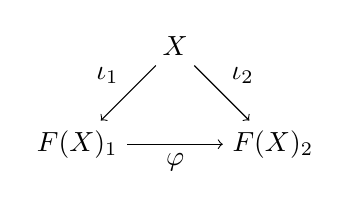
\begin{tikzpicture}[node distance = 5em]
   \node (X) {$X$};
   \node[below left of = X] (FX1) {$F(X)_1$};
   \node[below right of = X] (FX2) {$F(X)_2$};
   \draw[->] (X) to node[above left] {$\iota_1$} (FX1);
   \draw[->] (X) to node[above right] {$\iota_2$} (FX2);
   \draw[->] (FX1) to node[below] {$\varphi$} (FX2);
  \end{tikzpicture}
 \end{center}
 We will therefore always talk about \emph{the} free $k$-Lie algebra over $X$.
\end{rem}


\begin{lem}\label{lem: existince of free Lie algebras}
 Let $X$ be a set. Then there exists a free Lie algebra over $X$.
\end{lem}
\begin{proof}
 Let $A(X)$ be the free (unitary and associative) $k$-algebra over $X$ (which can be constructed as $T(kX)$, i.e.\ the tensor algebra over the free vector space $kX$ with basis $X$). Let $F(X)$ be the Lie subalgebra of $A(X)$ generated by $X$, i.e.
 \[
  F(X) = \bigcap \{\g \mid \text{$\g \subseteq A(X)$ is a Lie subalgebra with $X \subseteq \g$}\}.
 \]
 Let $\g$ be a $k$-Lie algebra and $\phi \colon X \to \g$ a map. By the universal property of the free $k$-algebra the map $\phi$ induces a homomorphism of $k$-algebras $\theta \colon A(X) \to \Ue(\g)$ making the following diagram commute, where the vertical maps are the canonical inclusions:
 \tikzsetnextfilename{construction_of_free_Lie_algebra}
 \begin{center}
  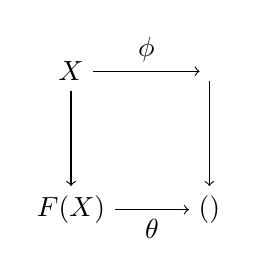
\begin{tikzpicture}[node distance = 5em]
   \node (X) {$X$};
   \node[right of = X] (g) {$\g$};
   \node[below of = X] (FX) {$F(X)$};
   \node[below of = g] (Ug) {$\Ue(\g)$};
   \draw[->] (X) to node[above] {$\phi$} (g);
   \draw[->] (FX) to node[below] {$\theta$} (Ug);
   \draw[->] (X) to (FX);
   \draw[->] (g) to (Ug);
  \end{tikzpicture}
 \end{center}
 As $\theta(X) = \phi(X) \subseteq \g$ it follows that $X \subseteq \theta^{-1}(\g)$. Because $\theta^{-1}(\g)$ is a Lie subalgebra of $F(X)$ containing $X$ it follows that $\theta^{-1}(\g) = F(X)$ and therefore $\theta(F(X)) \subseteq \g$. Hence $\theta$ restricts to a map $\Phi \colon F(X) \to \g$. Because $\theta$ is a homomorphism of $k$-algebras it is in particular a homomorphism of Lie algebras and therefore the same goes for $\Phi$. This shows the existence.
 
 For the uniqueness notice that $F(X)$ is by definition generated by $X$ and hence any homomorphism of Lie algebras $\Psi \colon F(X) \to \g$ is uniquely determinad by the restriction $\Psi|_X$.
\end{proof}


\begin{rem}
 The universal enveloping algebra is used in the proof of Lemma \ref{lem: existince of free Lie algebras} to ensure that any Lie algebra can be embedded into a $k$-algebra as a Lie subalgebra.
\end{rem}


\begin{rem}
 Using the concept of free Lie algebras one can define Lie algebras by giving a set of generators $X$ and a set of relations $R \subseteq F(X)$. As an example the Lie algebra $\sll(k)$ can be defined by the generators $R \coloneqq \{e,h,f\}$ with $e$, $h$, $f$ being pairwise different and the relations $R = \{[h,e]-2e, [h,f]+2f, [e,f]-h\}$, which can also be written as $[h,e] = 2e$, $[h,f] = -2f$ and $[e,f] = h$ as usual.
 
 More generally $\sll_{n+1}(k)$ for $n \geq 1$ can be defined as the Lie algebra generated by the $3n$ elements $\{e_i, f_i, h_i \mid i = 1, \dotsc, n\}$ together with the relations
 \begin{align*}
  [h_i, h_j] &= 0, \\
  [h_i, e_j] &= a_{ij} e_j, \\
  [h_i, f_j] &= -a_{ij} f_j, \\
  [e_i, f_j] &= \delta_{ij} h_i,
 \end{align*}
 for all $i,j = 1, \dotsc, n$ and
 \[
  \ad(e_i)^{1-a_{ij}}(e_j) = 0
  \quad\text{and}\quad
  \ad(f_i)^{1-a_{ij}}(f_j) = 0
  \quad \text{for $1 \leq i \neq j \leq n$},
 \]
 where the numbers $a_{ij}$ are for all $i,j = 1, \dotsc, n$ defined as
 \[
  a_{ij} =
  \begin{cases}
   \phantom{-}2 & \text{if $i = j$}, \\
             -1 & \text{if $|i-j| = 1$}, \\
   \phantom{-}0 & \text{otherwise}.
  \end{cases}
 \]
\end{rem}






























%\subsection{Hopf algebra structure}


\subsection{Casimir elements and operators}
For this subsection we additionaly assume that $\g$ is finite-dimensional. We also fix some bilinear form $\beta \colon \g \times \g \to k$ which is associative and non-degenerate.


\begin{defi}\label{defi: definition of Casimir element}
 Let $\varphi_1 \colon \g \otimes \g^* \to \End_k(\g)$ and $\varphi_2 \colon \g \to \g^*$ be the isomorphisms of vector spaces defined by
 \[
  \varphi_1(x \otimes \phi)(y) = \phi(y) x
  \quad\text{and}\quad
  \varphi_2(x) = \beta(x, \cdot)
  \quad\text{for all $x,y \in \g$ and $\phi \in \g^*$}.
 \]
 Then the image of $1$ under the map
 \begin{equation}\label{eqn: Casimir without coordinates}
  k
  \xrightarrow{\lambda \mapsto \lambda \id_\g}
  \End_k(\g)
  \xrightarrow{\varphi_1^{-1}}
  \g \otimes \g^*
  \xrightarrow{\id_\g \otimes \varphi_2^{-1}}
  \g \otimes \g
  \xrightarrow{x \otimes y \mapsto x y}
  \Ue(\g)
 \end{equation}
 is called the \emph{Casimir element of $\beta$} and denoted by $C_\beta$.
\end{defi}


\begin{lem}
 The Casimir element $C_\beta$ in central in $\Ue(\g)$, i.e.\
 \[
  x C_\beta = C_\beta x \quad \text{for every $x \in \Ue(g)$}.
 \]
\end{lem}
\begin{proof}
 Let $\varphi_1$ and $\varphi_2$ as in Definition \ref{defi: definition of Casimir element}.
 
 Because $\Ue(\g)$ is generated by $\g$ as a $k$-algebra it sufficies to show $C_\beta$ commutes with every $x \in \g$. Hence it is to show that
 \[
  [x,C_\beta] = 0 \quad \text{for every $x \in \g$},
 \]
 where $[\cdot,\cdot]$ denotes the Lie bracket in $\Ue(\g)$. To see this notice that in \eqref{eqn: Casimir without coordinates} every map is a homomorphism of representations of $\g$, where $\g$ acts trivially on $k$, i.e. $x.\lambda = 0$ for every $x \in \g$ and $\lambda \in \g$.
 
 That the first map $k \to \End_k(\g)$ is a homomorphism of representations follows from the fact that $\g$ acts trivially on $k$ and also trivially on the one-dimensional subspace $k \id_\g \subseteq \End_k(\g)$.
 
 That $\varphi_1$ is an isomorphism of representations is known from Propositon \ref{prop: list of homomorphism of representations}.
 
 That the third map $\g \otimes \g^* \to \g \otimes \g$ is a homomorphism of representations follows from Proposition \ref{prop: list of homomorphism of representations}, because the identity $\id_\g$ is a homomorphism of representations and and the isomorphism $\varphi_2$ is one by the associativity of $\beta$, as seen in Lemma \ref{lem: associative bilinear form induces homomorphism of representations}.
 
 That the fourth map $\psi \colon \g \otimes \g \to \Ue(\g), x \otimes y \mapsto xy$ is a homomorphism of representations follows from direct calculation, because for all $x,y,z \in \g$
 \begin{align*}
  \psi(x.(y \otimes z))
  &= \psi((x.y) \otimes z + y \otimes (x.z))
  = (x.y)z + y(x.z) \\
  &= [x,y]z + y[x,z]
  = xyz - yxz + yxz - yzx
  = xyz - yzx \\
  &= [x,yz]
  = x.(yz)
  = x.\psi(y \otimes z).
 \end{align*}
 
 Because every map in \eqref{eqn: Casimir without coordinates} is a homomorphism of representations it follows that their composition $\phi \colon k \to \Ue(\g)$ is also a homomorphism of representations. Definition \ref{defi: definition of Casimir element} is then equivalent to $\phi(1) = C_\beta$. Because $\g$ acts trivially on $k$ and $\phi$ is a homomorphism of representations it follows that $\g$ also acts trivially on the span of $C_\beta$. In particular
 \[
  0 = x.C_\beta = [x,C_\beta] \quad \text{for every $x \in \g$}.
  \qedhere
 \]
\end{proof}


\begin{lem}[Casimir in coordinates]
 Let $x_1, \dotsc, x_n$ be a basis of $\g$ and $x^1, \dotsc, x^n$ the dual basis of $\g$ with respect to $\beta$, i.e.\ $\beta(x_i, x^j) = \delta_{ij}$ for all $i,j = 1, \dotsc, n$. Then
 \[
  C_\beta = \sum_{i=1}^n x_i x^i.
 \]
\end{lem}
\begin{proof}
 Let $\varphi_1$ and $\varphi_2$ as in Definition~\ref{defi: definition of Casimir element}. In \eqref{eqn: Casimir without coordinates} $1$ is mapped to $\id_\g$, which is then mapped to $\sum_{i=1}^n x_i \otimes x_i^*$, where $x_1^*, \dotsc, x_n^*$ denotes the dual basis of $\g^*$. As $\varphi_2(x^i) = x_i^*$ it follows that $\sum_{i=1}^n x_i \otimes x_i^*$ is then mapped to $\sum_{i=1}^n x_i \otimes x^i$, which is then further mapped to the element $\sum_{i=1}^n x_i x^i$ in $\Ue(\g)$.
\end{proof}















